
%----------------------------------------------------------------------------------------
%	PREAMBUŁA
%----------------------------------------------------------------------------------------

\documentclass[12pt]{article}
\usepackage[polish]{babel}
\usepackage[T1]{fontenc}
\usepackage{polski}
\usepackage[utf8]{inputenc}
\usepackage{amsmath}
\usepackage{graphicx}
\usepackage{fancyhdr}
\usepackage{float}
\usepackage{graphicx}
\usepackage{hyperref}
\usepackage{verbatim}
\usepackage{listings}

\title{Dokumentacja}
\author{Aleksandra Poręba}

\graphicspath{{static/}} 

\makeatletter
\let\thetitle\@title
\let\theauthor\@author
\let\thedate\@date
\makeatother



 
%----------------------------------------------------------------------------------------
%	STRONA TYTUŁOWA
%----------------------------------------------------------------------------------------
\begin{document}
\begin{center}
\textsc{\normalsize Wydział Fizyki i Informatyki Stosowanej}\\[2.0cm] 

\includegraphics[scale = 1]{logo.png}\\[1cm] 
\textsc{\Large Dokumentacja projektu}\\[0.4cm] 

{ \huge \bfseries \LARGE{Grafowa baza danych POC} }\\[1cm] 

\flushright \Large Aleksandra Poręba \\ nr. indeksu 290514

\vfill 

\center {\today}\\[2cm] 

\pagebreak 

\end{center}

%----------------------------------------------------------------------------------------
%	SPIS TREŚCI
%----------------------------------------------------------------------------------------
\tableofcontents
\pagebreak

%----------------------------------------------------------------------------------------
%	ZAWARTOŚĆ
%----------------------------------------------------------------------------------------

\pagestyle{fancy}
\fancyhf{}

\rhead{\theauthor}
\lhead{\thetitle}
\cfoot{\thepage}

\section{Opis działania aplikacji}
Celem aplikacji było zademonstrowanie użycia grafowej bazy danych.

Aplikacja udostępnia możliwość wyszukiwania najszybszego połączenia pomiędzy przystankami. Użytkownik ma możliwość dodawania własnych przystanków i relacji między nimi, usuwanie ich, a także modyfikację.

Na stronie głównej, przestawionej na rysunku \ref{fig:rys1}, przedstawiona jest lista wszystkich dostępnych przystanków w aplikacji.

\begin{figure}
\begin{center}
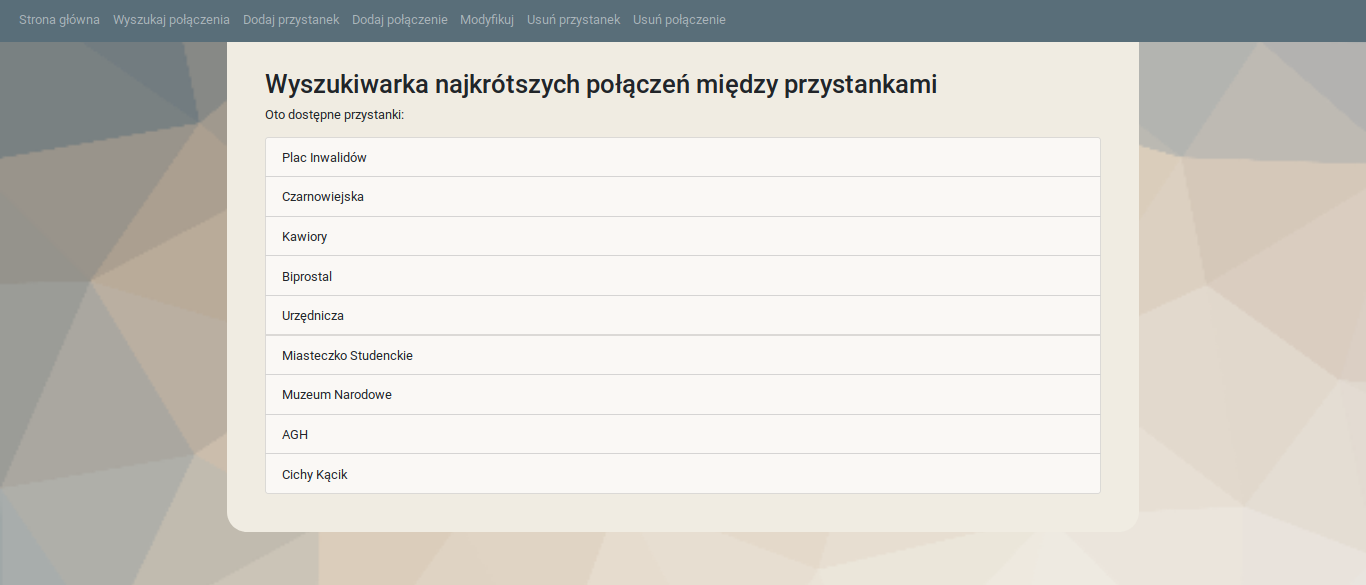
\includegraphics[width=14cm]{strona.png} 
\caption{Strona główna aplikacji} \label{fig:rys1}
\end{center}
\end{figure}

Przemieszczanie się po stronie odbywa się za pomocą paska nawigacji.

\subsection{Dodawanie}
W aplikacji możemy dodawać zarówno przystanki jak i połączenia. Jeśli chcemy dodać przystanek należy w formularzu podać jego nazwę oraz adres. 

Aby utworzyć nowe połączenie pomiedzy punktami, należy wybrać dwa odpowiednie przystanki z listy, podać numer autobusu (może być też tramwaju), którym możemy odbyć tą trasę oraz szacowany czas w minutach.

Aplikacja jest zabezpieczona przed dodaniem nieprawidłowych danych, takich jak puste wartości, za krótka nazwa ulicy, czy wybór takich samych przystanków.

\subsection{Modyfikacja}
W zakładce "Modyfikuj" mamy możliwość zmienienia danych dotyczących przystanku. Po wybraniu nazwy punktu, którego chcemy edytować, zostaje otworzony formularz do zmiany danych.

\subsection{Usuwanie}
Aplikacja udostępnia możliwość usunięcia przystanków razem z wszystkim połączeniami do nich, oraz pojedynczych połączeń. Aby tego dokonać należy wybrać interesujące użytkownika nazwy z listy.

\subsection{Wyszukiwanie}
W zakładce "Wyszukaj połączenia" użytkowanik może wyszukać najszybszą trasę pomiędzy dwoma przystankami. W rezultacie zostaje wyświetlona tabela z kolejnymi przystankami, numerem autobusu (tramwaju), którym możemy dojechać na dany przystanek, oraz ile czasu podróży już mineło, od jej rozpoczęcia.

\section{Typy danych}

\section{Wykorzystane technologie}
Aplikacja została zrealizowana za pomocą mikrofameworka Flask w Pythonie 3. Dostęp do bazy danych jest realizowany przez bibliotekę neo4jrestclient, wysyłająca zapytania do serwera REST bazy Neo4j. Połączenie jest realizowane przez HTTP REST. Zapytania do bazy danych zostały napisane w języku zaptań Cypher. Baza danych jest dostarczana przez graphenedb, jest to baza Neo4j w chmurze, hostowana na Heroku.

Do oprawy graficznej strony został użyty framwork Bootstrap4.

Aplikacja znajduje się w środowisku chmurowym Heroku pod adresem:
\url{https://pure-river-73041.herokuapp.com/}.


\section{Bibliografia}
\href{https://devcenter.heroku.com/articles/graphenedb#using-with-python-and-neo4j-rest-client}{Using with Python and Neo4j Rest Client}
\\
\href{https://neo4j.com/docs/cypher-manual/current/}{The Neo4j Cypher Manual v3.5}
\\
\href{https://neo4j-rest-client.readthedocs.io/en/latest/info.html}{neo4j-rest-client’s Documentation}
\\
\href{https://neo4j.com/docs/graph-algorithms/current/}{The Neo4j Graph Algorithms User Guide v3.5}

\end{document}